The exploration vs. exploitation dilemma is still an open problem in RL. Classic exploration approaches like $\epsilon$-greedy or Boltzman work well for simple problems, but they do not address temporally extended (or deep) exploration. In Chapter 2 we discussed some classic and modern, model-free and model-based algorithms that do efficient or deep exploration. In this chapter we propose a new model-free approach to the exploration vs. exploitation tradeoff. \emph{Particle Q Learning} explicitly expresses the uncertainty about the Q-value estimates by maintaining Q-value distributions and uses them to make better decisions during the learning process. We approximate the Q-value distribution by attaching fixed weights to variable (parametrized) locations. We call these parametrized locations, \emph{particles}, hence the name. This way we attempt to estimate the quantiles of the target distribution. \par
We begin in Section ~\ref{sec:q_value_distributions} where we define our approximation of the Q-distribution and derive some interesting results. In Section ~\ref{sec:action_selection} we propose two possible policies that use the Q-distributions as defined in Section ~\ref{sec:q_value_distributions}. Finally, in Section ~\ref{sec:updating_q_distributions},  we discuss how to maintain the distributions from samples of experience $(s,a,r,s')$.

\section{Q Value Distributions} \label{sec:q_value_distributions}
A reinforcement learning agent needs to do exploration because he is uncertain about the true Q-values of the actions. Indeed, this uncertainty is the reason for doing learning in the first place. An agent that is certain about the Q-value estimates of all the action has no reason to explore, since it does not expect there to be a better policy to discover. It seams reasonable to us, that decisions whether to explore new actions or to exploit the current best ones, should be done based on how uncertain the agent is about the Q-values. Therefore this uncertainty should be expressed explicitly in an RL agent.\par
We represent the uncertainty we have about the Q-value estimates, using a \emph{Q-distribution}, a probability distribution over the possible values that the Q-value might take. Formally, let $R_{s,a}$ be a random variable that denotes the total discounted reward received when action $a$ is executed in state $s$ and then an optimal policy is followed. We note that $Q^*(s,a)=\mathbb{E}[R_{s,a}]$. The objective of the agent is to learn $\mathbb{E}[R_{s,a}]$, and not approximate the whole distribution of $R_{s,a}$, as the knowledge of the expectation of the return is sufficient to act optimally. In this section we will review the proposed Q-value distribution.
\subsection{Particle Q Distribution}
We will denote with $Q(s,a)$ the random variable representing the expected cumulative reward from $(s,a)$ following the optimal policy. To approximate this distribution we will use a parametric model, parametrized over $N$ locations, which we call particles, associated to fixed weights $\frac{1}{N}$. We indicate with $\mathcal{Q}(s,a)$ the set of particles associated to $(s,a)$ ($\vert \mathcal{Q}(s,a) \vert =N$):
\begin{equation}
\mathcal{Q}(s,a)={x^i_{s,a} \qquad i=1, \ldots,N}.
\end{equation}
where $x^i_{s,a}$, is the $i$th particle of the state action pair $(s,a)$. We will assume, without loss of generality, $x_1 \leq x_2 \ldots \leq x_N$. This way, the Q-distribution is approximated by the following \emph{mixture of deltas}:
\begin{equation}
	p(x \vert s,a)=\sum_{i=1}^{N} \frac{1}{N} \delta(x-x^i_{s,a}).
	\label{eq:particle_distribution}
\end{equation}
The c.d.f is given by:
\begin{equation}
\hat{F}(x \vert s,a) = \sum_{i=1}^{N} \frac{1}{N} H(x-x^i_{s,a}),
\end{equation}
where H is the Heaviside step function, defined as:
\begin{equation}
	H(x) = \begin{cases}
    			1 & x \ge 0 \\
                0 & x < 0
    		\end{cases}.
\end{equation}
Using this parametrized distribution, we try to estimate the quantiles of the Q-distribution.\par
It is important to note the fundamental difference between maintaining a distribution of the return $R_{s,a}$, and the distribution of the Q-values, $\mathbb{E}[R_{s,a}]$. While the return $R_{s,a}$ has an intrinsic randomness, which might come from different factors  like the stochasticity of the underlying model of the MDP or the randomness of the reward function, the Q-values are the expected value of this return. We keep a distribution of the Q-values to represent our uncertainty about the current estimate. We expect that at the end of the learning process this distribution shrinks to the real Q-value. On the other hand, when maintaining the distribution of the return, the distribution will remain wide to represent the intrinsic randomness of the MDP. Figure ~\ref{fig:q_distribution_behaviour} shows the expected behavior of the learning process. The distribution will start flat (given that the prior is initialized that way). As the learning process continues, the agent observes a sequence of values from $\mathbb{E}[R_{s,a}]$ and updates its belief. As the learning process continues, the distribution should get progressively more peaked and the agent becomes more certain about the actual Q-value.
\begin{figure}
 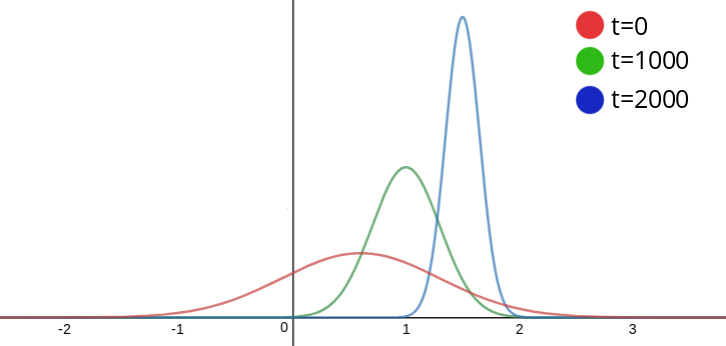
\includegraphics[width=\linewidth]{q_distribution_behaviour.jpg}
 \caption{Behaviour of the Q-distribution over time.}
 \label{fig:q_distribution_behaviour}
\end{figure}
\subsection{Sample Mean Distribution}
We consider a collection of random variables $\{X_i\}_{i=1}^m$ and $I \in \{1,\dots,m\}$ a random index; we aim to estimate the mean $\widehat{\mu}_Y$ of $Y = X_{I}$ assuming to have estimations of the means $\widehat{\mu}_{X_i}$ of $X_i$. We assume $I \sim \rho$ where $\Pr(I = i) = \xi_i$ unknown. Standard Monte Carlo estimation would sample $I$ from $\rho$ distribution $N$ times and perform the estimate:
\begin{equation}
	\widehat{\mu}_{Y}^{MC} = \frac{1}{N} \sum_{j=1}^N \widehat{\mu}_{X_{I_j}}, \quad I_j \sim \rho.
\end{equation}
Suppose to know the distribution of the sample means $\widehat{\mu}_{X_i} \sim \nu_i$. Which is the best approximating distribution for the sample mean? In~\cite{NIPS2017_7149}, in the context of Gaussian processes, the authors claim that by tacking the convolution of the single distributions $\nu_i$ properly weighted with $\xi_i$ would underestimate the uncertainty on $\widehat{\mu}_{Y}^{MC}$. Indeed, if $m\rightarrow \infty$ the uncertainty would be null. Contrary, we could find the distribution $\nu$ minimizing:
\begin{equation}
	\mathcal{L}_d^p (\nu) = \mathbb{E}_{I \sim \rho} \left[ d(\nu, \nu_I)^p \right],
\end{equation}
where $d$ is a suitable distribution divergence and $p>0$. $\nu^* = \argmin_{\nu \in \mathcal{N}} \mathcal{L}_d^p (\nu)$ is called \emph{Barycenter}~\cite{journals/siamma/AguehC11} of $\{\nu_i\}_{i=1}^m$ \wrt divergence $d$. The same loss function can be computed from samples as:
\begin{equation}
	\widehat{\mathcal{L}}_d^p (\nu)  = \frac{1}{N} \sum_{j=1}^N d(\nu, {\nu_{I_j}}), \quad I_j \sim \rho.
\end{equation}
If $\nu = \nu_{\theta}$ belongs to $\mathcal{N}_{\Theta} = \{ \nu_{\theta}: \theta \in \Theta \subseteq \mathbb{R}^d \}$ a parametrized distribution space differentiable in $\theta$ and $d$ is differentiable \wrt the first argument we can find the parameter $\theta^*$ via stochastic gradient descent:
\begin{equation}
	\theta^{(t+1)} = \theta^{(t)} - \alpha \nabla_\nu d(\nu, {\nu_{I}}) \nabla_{\theta} \nu_{\theta^{(t)}}, \quad I \sim \rho.
\end{equation}
\subsection{Approximation of a distribution function with mixture of delta functions}
We consider a c.d.f. $F(x)$ that we want to approximate with:
\begin{equation}
	\widehat{F}_n(x) = \frac{1}{n} \sum_{j=1}^n w_j H(x-x_j).
\end{equation}
We start considering the case in which $w_j$ are fixed.
We need to determine $x_j$ such that the distance between the distribution of $F(x)$ and $\widehat{F}_n(x)$ is minimal.Clearly, using discontinuous distributions the classical divergences like KL or TV are inappropriate (they are always maximal). We resort to the Wasserstein metric. We use $W_2(F, \widehat{F}_n)$ as metric.

\begin{theorem}
	Let $F(x)$ a c.d.f. of r.v. $X$ s.t. $X \in [a,b]$ a.s.. Then, the 2-Wasserstein distance $W_2(F, \widehat{F}_n)$ has the unique minimizer:
    \begin{equation}
    	\widehat{x}_j = \frac{1}{|I_j|} \int_{I_j} F^{-1}(t) \mathrm{d} t, \quad j=1,2,\dots, n,
    \end{equation}
    where $I_j=[t_{j-1}, t_j)$, $t_0 = 0$ and $t_j = \sum_{k=1}^j w_j$. In this case, the 2-Wasserstain distance can be bounded as:
    \begin{equation}
    	W_2(F, \widehat{F}_n) \le \frac{(b-a)^2}{4} \max_{j=1,2,\dots,n} |I_j|.
    \end{equation}
\end{theorem}

\begin{proof}
	Let us first compute the quantile function $\widehat{F}_n^{-1}$:
    \begin{equation}
    	\widehat{F}_n^{-1}(t) = \sum_{j=1}^n x_j \mathds{1}_{I_j}(t),
    \end{equation}
    where $\mathds{1}$ is the indicator function. The 2-Wasserstin distance can be written as:
    \begin{align*}
    	W_2^2(F, \widehat{F}_n) & = \int_0^1 \left( F^{-1}(x) - F_n^{-1}(x) \right)^2 \mathrm{d} t = \\
        & = \sum_{j=1}^n \int_{I_j} \left( F^{-1}(x) - x_j \right)^2  \mathrm{d} t. 
    \end{align*}
    We take the derivative \wrt $x_j$ and we get:
    \begin{equation}
    	\frac{\partial W_2^2}{\partial x_j} = -2 \int_{I_j} \left( F^{-1}(x) - x_j \right)  \mathrm{d} t = 0.
    \end{equation}
    From which the first result follows. Let us now observe, since $F^{-1}$ is monotonically increasing, that for every $j$:
    \begin{align*}
    	\int_{I_j} \left(F^{-1}(x) - \widehat{x}_j\right)^2 \mathrm{d} t & \le \int_{I_j} \left(F^{-1}(x) - \frac{F^{-1}(t_j) - F^{-1}(t_{j-1}) }{2}\right)^2 \mathrm{d} t \le \\
        & \le\frac{1}{4} \int_{I_j} \left( (F^{-1}(x) - F^{-1}(t_j)) +  (F^{-1}(x) - F^{-1}(t_{j-1})) \right)^2 \mathrm{d} t \le \\
        & \le \frac{1}{4} \int_{I_j} \left( (F^{-1}(x) - F^{-1}(t_j)) -  (F^{-1}(x) - F^{-1}(t_{j-1})) \right)^2 \mathrm{d} t \le \\
       & \le\frac{1}{4} \int_{I_j} \left( F^{-1}(t_j) - F^{-1}(t_{j-1} \right)^2 \mathrm{d} t \le \\
       & \le \frac{1}{4} |I_j| \left( F^{-1}(t_j) - F^{-1}(t_{j-1}) \right)^2.
    \end{align*}
    Let us call $\Delta_j = F^{-1}(t_j) - F^{-1}(t_{j-1})$, the error can be bounded overall as:
    \begin{align*}
    	W_2^2(F, \widehat{F}_n) & \le \frac{1}{4}  \sum_{j=1}^n |I_j| \Delta_j ^2 \le \\
        & \le \frac{1}{4} \max_j |I_j| \sum_{j=1}^n \Delta_j ^2 \le \\
        & \le \frac{1}{4} \max_j |I_j| \left( \sum_{j=1}^n \Delta_j \right) ^2 \le \\
        & \le \frac{1}{4} \max_j |I_j| \left(b-a\right) ^2,
    \end{align*}
    where we used Cauchy–Schwarz inequality ~\cite{Steele:2004:CMC:993490} in the last passage, observing that $\Delta_j \ge 0$ from the monotonicity of $F^{-1}$.
\end{proof}

For the case of uniform $w_j = 1/n$ the result reduces to:
\begin{equation}
	W_2^2(F, \widehat{F}_n) \le \frac{(b-a)^2}{4N}.
\end{equation}
Thus if $N\rightarrow \infty$ the error goes to zero. Up to now we considered the error introduced by representing a given distribution with a mixture of deltas. 

It is interesting to investigate the properties of the approximating distribution $\widehat{F}_n$

\begin{prop}
	Let $\widehat{F}_n$ be the approximating c.d.f. of $F$ as defined before. Then it holds that:
    \begin{equation}
    	\ev_{\widehat{F}_n} [X] = \ev_{F} [X].
    \end{equation}
\end{prop}

\begin{proof}
	We first observe that by making the substitution $x = F^{-1}(t)$ we have the identity:
    \begin{equation}
    	\int_{I_j} F^{-1}(t) \mathrm{d} t = \int_{F^{-1}(t_{j-1})}^{F^{-1}(t_{j})} x f(x) \mathrm{d}x.
    \end{equation}
    Therefore:
    \begin{align*}
    	\ev_{\widehat{F}_n} [X] & =\int_a^b x \widehat{f}_n(x) \mathrm{d}x = \\
        & = \sum_{j=1}^n w_j x_j = \\
        & = \sum_{j=1}^n w_j \frac{1}{|I_j|} \int_{I_j} F^{-1}(t) \mathrm{d} t = \\
        & = \sum_{j=1}^n \int_{I_j} F^{-1}(t) \mathrm{d} t = \\
        & = \sum_{j=1}^n \int_{F^{-1}(t_{j-1})}^{F^{-1}(t_{j})} x f(x) \mathrm{d}x = \\
        & = \int_{a}^{b} x f(x) \mathrm{d}x = \ev_{F} [X].
    \end{align*}
\end{proof}

Thus, our approximation preserves the mean. This does not hold in general for the other moments.


Now we move to the problem of finding a proper Wasserstein barycenter.
\subsection{Wasserstein barycenter} 
We represent the distribution of the sample mean by means of uniform ($w_j=1/n$) mixtures of Dirac deltas. Our problem is to determine the 2-Wasserstein barycenter of a set of mixtures differently weighed with the same number of components. 
\begin{equation}
\label{eq:problem}
	\widehat{\mathbr{x}} = \argmin_{\mathbr{x}} \sum_{i=1}^m \xi_i W_2^2(F_X, F_{Y_i}),
\end{equation}
where $f_X(x) = 1/n \sum_{j=1}^n \delta(x-x_j)$ and $f_{Y_i}(x) = 1/n \sum_{j=1}^n \delta(x-y_{ij})$. We will prove that this problem has a closed form solution (remember that we assume to consider the $x$ and $y$ sorted):

\begin{theorem}
	The unique solution of the problem~\ref{eq:problem} is given by:
    \begin{equation}
    	\widehat{\mathbr{x}} = \mathbr{Y} \mathbr{\xi},
    \end{equation}
    where $\mathbr{Y} = (\mathbr{y}_1 | \dots | \mathbr{y}_m)$.
\end{theorem}

\begin{proof}
	We observe that, since all weights are $w_j = 1/n$, the relevant quantiles are the same for all involved distributions, \ie $1/n$. As a consequence, fixing $i$, we can easily compute the 2-Wasserstein distance as:
    \begin{equation}
    	W_2^2 (F_X, F_{Y_i}) = \frac{1}{n} \sum_{j=1}^n (x_j - y_{ij})^2 = \frac{1}{n} \| \mathbr{x} - \mathbr{y}_i \|^2_2.
    \end{equation}
    Thus, the objective function can be written as:
    \begin{equation}
    	\mathcal{L}(\mathbr{x}) = \frac{1}{n} \sum_{i=1}^m \xi_i \| \mathbr{x} - \mathbr{y}_i \|^2_2.
    \end{equation}
    This is a convex function, all it takes is to vanish the gradient:
    \begin{equation}
    	\nabla_{\mathbr{x}} \mathcal{L}(\mathbr{x}) = \frac{2}{n} \sum_{i=1}^m \xi_i (\mathbr{x} - \mathbr{y}_i) = 0 \implies \mathbr{x} =  \sum_{i=1}^m \xi_i \mathbr{y}_i = \mathbr{Y} \mathbr{\xi},
    \end{equation}
    where $\mathbr{Y} = (\mathbr{y}_1 | \dots | \mathbr{y}_m)$.
\end{proof}

Clearly, in reality the probabilities $\xi_i$ are not known and we want to avoid to estimate them separately (this would bring to a model-based approach as the $\xi_i$ are the probabilities defining the transition model). For this purpose we look at the objective function as an expected value:
\begin{equation}
	 \mathcal{L}(\mathbr{x}) = \ev_{I \sim \rho} [W_2^2(F_X, F_{Y_I})] = \frac{1}{n} \sum_{j=1}^n \ev_{I \sim \rho} [(x_j - y_{Ij})^2].
\end{equation}
Therefore we can employ a SGD update rule for the $x_j$.
\begin{equation}
	\mathbr{x}^{(t+1)} = \mathbr{x}^{(t)} - \alpha \nabla_{\mathbr{x}} \widehat{\mathcal{L}}(\mathbr{x}^{(t)} ) =  \mathbr{x}^{(t)} - \frac{2\alpha}{n} (\mathbr{x}^{(t)} -\mathbr{y}_{i^{(t)}} )
\end{equation}

It is simple to prove that the Wasserstein barycenter satisfies the following relation:
\begin{equation}
	\ev_{F_X}[X] = \ev_{I \sim \rho} \ev_{F_{Y_I}} [Y_I].
\end{equation}

\section{Action Selection} \label{sec:action_selection}
The classical approach to exploration, applied in $\epsilon$-greedy or Boltzman exploration, is selecting actions with the highest Q-value estimate or randomly selecting an action based on the number of timesteps of learning performed. The heuristics of this is that, at the beginning of the learning process, the Q-value estimates are unreliable and exploration is done randomly. An exploration schedule is defined, based on the timesteps, so that as the learning progresses, exploration is done less and less, until it reaches 0 and the agent exploits the Q-values it has learned. This is done because there is no measure of the uncertainty of the Q-value estimates. \par 
In this section we will discuss two methods of choosing action based on the uncertainty of the Q-value estimates. The first one is an adaptation of Myopic VPI, used in ~\cite{Dearden98bayesianq-learning}. The idea is that, by using the Q-distributions, the agent can answer the exploration vs. exploitation dilemma explicitly, by weighting the benefits of exploiting the current best actions, versus the benefits of exploring new actions that give more information on the task at hand. In the limit, when the Q-distributions shrink to the true Q-values, Myopic VPI turns in a simple greedy policy that chooses the best actions. The second method, \emph{Weighted Policy}, choses actions based on the probability of each action of being maximal. Since we maintain distributions over Q-values, we can explicitly calculate the probabilities of each action to be optimal, and then execute the action with the highest probability.
\subsection{VPI Policy}
When the agent selects an action, we would like to strike a balance between present performance, the current optimal action based on our estimates, and future performance, actions that might turn out to be optimal in the future. This is in fact the essence of the exploration vs. exploitation dilemma. In our proposed approach, the agent maintains a Q-distribution for each state-action pair, $(s,a)$. Using these distributions, we can calculate the value of perfect information (VPI) ~\cite{4082064,Russell:1991:RTS:110787}, as in ~\cite{Dearden98bayesianq-learning}. This information is used to calculate the \emph{value of exploration}, hence balancing present and future performance.\par
As an example, consider Figure ~\ref{fig:q_distributions}. The Q-distributions of 3 different actions are shown. Choosing actions based on the mean of each distribution would result in a simple greedy policy, since the mean of the distribution is our estimate of $\mathbb{E}[R_{s,a}]$. Obviously action 1 is a bad choice. The distribution is pretty confident about the low return of this action, so the action is well explored. Consequently the likelihood of action 1 to be optimal is low, so by executing it we  will (very likely) lose in current performance and also will not learn any valuable information. Considering the means of the distributions action 3 is the current optimal action. Also the variance of its distribution is low, so we are confident of it's high return. Action 2 on the other had is certainly a candidate to be executed. The current cost of executing action 2, instead of the current optimal, is low, since the means of the two distributions are close. The second Q-distribution also has a high variance, which means we have low confidence on its real return, and exploring this action might actually be beneficial in the future. VPI measures the value of each action based on these kind of considerations.
\begin{figure}
 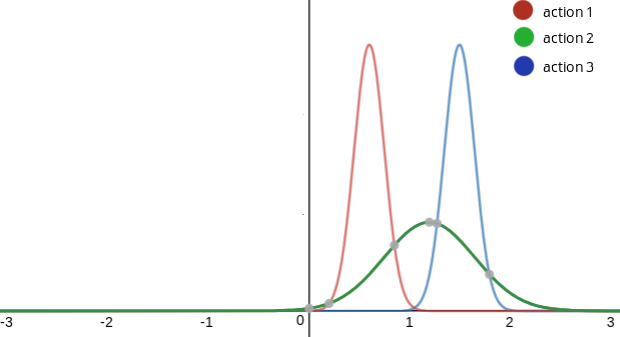
\includegraphics[width=\linewidth]{q_distributions.jpg}
 \caption{Q-distributions of 3 different actions.}
 \label{fig:q_distributions}
\end{figure}
To select which action to execute, the VPI is computed for each possible action in the current state. However, we have to consider also the cost of executing action $a$ instead of action $a_1$, the current optimal action. To select the action we have to consider the value VPI minus the difference in the expected value of $a$ and $a_1$. Formally, we choose the action that maximizes:
\begin{equation}
	VPI(s,a)- (\max_{a'} \mathbb{E}[Q(s,a')]- \mathbb{E}[Q(s,a)]).
\end{equation} 
Clearly, the expected value of the optimal action, $\max_{a'} \mathbb{E}[Q(s,a')$, is equal for all actions, so this strategy is equal to maximizing:
\begin{equation}
	VPI(s,a)+ \mathbb{E}[Q(s,a)].
\end{equation}
This way, the gain due to possible future observation is balanced with the cost of executing a current suboptimal action, instead of the current best one.\par
Computing the VPI can be thought as answering the question ``what would I be willing to pay to learn the true value, $v^*$, of this action''. If the information is worth a lot, then the information might be worth discovering through exploration. On the other hand, if the information is not worth a lot, it might be better to exploit the current optimal action. Let $q^*_{s,a}$ be the true expected value of action $a$ in state $s$. We first note that knowing the true value of the action is worth nothing is the current policy does not change ($VPI(s,a)=0$). Let $a_1$ be the current optimal action (\ie the action with the highest expected Q-value given the current information). Let $a_2$ be the action we currently believe is second best. If we learn that the true expected value of $a_1$ is higher than the expected value $a_1$, we have confirmed the current optimal policy, so we did not gain any new information. Note that the \emph{expectation} of the total discounted reward might have changed if we learned a new value for $a_1$, but the $actual$ expected discounted future reward is unchanged if we did not change our policy.  Similarly, if we learn the true value of some other action $a$, and we learn that the true value is still lower than the value of $a_1$, the new information has no value. \par 
We are left with two cases in which learning the true value of an action has some worth:
\begin{itemize}
\item When the new information shows that an action previously thought optimal is actually inferior to other actions,
\item When the new information shows that an action previously thought sub-optimal, is actually the optimal action.
\end{itemize} 
More formally, let $s$ be the current state, $a$ the action whose VPI is being calculated and $q_{s,a}$ a possible value of $Q^*(s,a)=\mathbb{E}[R_{s,a}]$. Let the two current best actions be $a_1$ and $a_2$. Then we can define the gain from learning that $a$ has expected value $q^*_{s,a}$ is ~\cite{Dearden98bayesianq-learning}:
\begin{equation}
	Gain_{s,a}(q^*_{s,a}) = \begin{cases}
    			\mathbb{E}[q_{s,a_2}]- q^*_{s,a}  & \text{if } a=a_1 \text{ and } q^*_{s,a}< \mathbb{E}[q_{s,a_2}] \\
                q^*_{s,a} - \mathbb{E}[q_{s,a_1}]  & \text{if } a \neq a_1 \text{ and  }q^*_{s,a}> \mathbb{E} [q_{s,a_1}] \\
                0 & \text{otherwise}
    		\end{cases}.
\end{equation}
Of course we do not have the value of $q^*_{s,a}$. Instead we have a Q-distribution over the value of $q^*_{s,a}$. So we can weight the gain of learning the true value of action $a$, $q^*_{s,a}$, with the probability of it being the true value according to the current Q-distribution, calculating the expected value of perfect information (EVPI) ~\cite{Dearden98bayesianq-learning} :
\begin{equation}
VPI(s,a)=\int_{-\infty}^{\infty} Gain_{s,a}(x) Pr(q_{s,a}=x) dx.
\label{eq:vpi_equation}
\end{equation}
In our case the Q-distriution is approximated using the particle distribution defined in (~\ref{eq:particle_distribution}). The integral in (~\ref{eq:vpi_equation}) turns into a sum over the particles as follows:
\begin{equation}
	VPI(s,a) = \begin{cases}
    			\sum_{x^k_{s,a} \leq \mathbb{E}[Q(s,a_2)]} \frac{1}{N}\left(\mathbb{E}[Q(s,a_2)]- x^k_{s,a}\right)  & \text{if } a=a_1 \\
                \sum_{x^k_{s,a} \geq \mathbb{E}[Q(s,a_1)]} \frac{1}{N}\left(x^k -\mathbb{E}[Q(s,a_1)]\right)  & \text{if } a \neq a_1 \\
    		\end{cases}.
\end{equation}
The value of perfect information estimate is used an a way of boosting the desirability of different actions. When the agent is confident about the value Q-value estimates VPI will go to zero and the VPI policy will turn to a simple greedy policy.
\subsection{Weighted Policy}
VPI policy tries to estimate the value of exploring a sub-optimal action, rather than exploiting the current best action. As Dearden et al. note in ~\cite{Dearden98bayesianq-learning}, this value of VPI is an optimistic assessment of the value of performing $a$. By executing $a$ we do not get perfect information about it's value, we just get one more training instance. We will now propose another policy that uses the Q-distributions maintained by our agent. \emph{Weighted policy} choses actions based on their probability of being optimal. Assuming that the Q-values of the different actions in state $s$ are independent (assumption that hardly holds in practice), the probability of  action $a$ to be optimal, $P(a= \argmax_{a'} Q(s,a'))$, is given by:
\begin{equation}
	\begin{split}
	P\left(a= \argmax_{a'} Q(s,a')\right) & = P\left(\forall a' \neq a, \prod Q(s,a) > Q(s,a')\right) \\
							   & = \int_{-\infty}^{\infty} P\left(Q(s,a)=x\right) \Pi_{a' \neq a} F_{a'}(x)dx
	\end{split},
	\label{eq:maximum_probability}
\end{equation}
where $F_{a'}(x)$ is the c.d.f. of the Q-distribution of action $a'$. Replacing the probabilities in (~\ref{eq:maximum_probability}), with our mixture of deltas distribution we get the following:
\begin{equation}
	P\left(a= \argmax_{a'} Q(s,a')\right)=\sum_{i=1}^{N} \frac{1}{N} \prod_{a' \neq a} \sum_{x_{a'}^j < x_a^i} \frac{1}{N}.
\end{equation}
Deriving the above formula is straightforward. The integral turns into a sum over the particles, for which $P(Q(s,a)=x^i_{s,a})=\frac{1}{N}$. 
\section{Updating the Q-distribution} \label{sec:updating_q_distributions}
In this section we will discuss how to update the Q-distributions maintained by the agent after executing a transition. We recall the agent maintains a distribution over Q-values , for each state-action pair, $(s,a)$, represented by a set of $N$ uniformly weighted particles. The problem at hand is how to move the set of particles $\mathcal{Q}(s,a)$ after observing local reward $r$. An obvious problem is that the distributions are over the Q-values whereas the agent observes samples from local reward, $R(s,a)$.
\par Suppose the agent is in state $s$, executes action $a$, and observes reward $r$ and next state $s'$. Let $R_{s'}$ be a random variable denoting the total sum of discounted reward from state $s'$ under an optimal policy. In this section we will see two methods to approximate the target distribution $R_{s'}$ and how to use to update the distribution of $Q(s,a)$.
\subsection{Sorted Update}
Suppose, after observing the transition $s,a,r,s'$, we have a set of $N$ particles , $\mathcal{Q}(s',a')$ representing our target distribution. The problem at hand is how to update the distribution of $Q(s,a)$ using this set of particles. The simplest idea would be to just add the new set of particles to the old set, building the set $\mathcal{Q}_{all}= \mathcal{Q}_{s,a} \cup \mathcal{Q}(s',a')$. The obvious problem with this approach is that the set would grow infinitely. We need to find the set of particles $\mathcal{Q}(s,a)$ that minimizes some sort of distance between the distribution represented from the set $\mathcal{Q}_{all}$. \par 
More formally, let $\mathcal{Q}^t(s,a)=x^t_i, \quad i=1,\ldots,N$ , $\mathcal{Q}'^t(s,a)=x'^t_i, \quad i=1,\ldots,N$ be the set of particles representing the prior and target distributions at step $t$. The set of particles minimizing the $W_2$ distance between the posterior and target distributions is given by:
\begin{equation}
	\label{eq:sorted_update}
	x^{t+1}_i \leftarrow x^{t}_i + \alpha (x'^{t}_i - x^{t}_i) \qquad i=1,\ldots,N , 
\end{equation}
where $\alpha$ is the learning rate. We recall that the set of particles are sorted. 
\subsection{Maximum Mean Updating}
\emph{Maximum mean updating} assumes the agent will follow the apparently optimal policy at state $s'$. Following this assumption, then $R_{s'}$ is distributed as $R_{s,a'}$ where $a'$ is the action with highest expected reward at state $s'$ ($a'=\argmax_{a} \ev[Q(s',a)])$. This means that to update the distribution of $Q(s,a)$ we can use the distribution of $Q(s',a')$, represented by the set of particles $\mathcal{Q}(s',a')$. Pseudocode of the algorithm is shown in Alg. ~\ref{alg:max_mean_updating}. 
\begin{algorithm}[H]
\begin{flushleft}
 \textbf{Input:} A transition $s,a,r,s'$, $\gamma \in [0,1]$, $\alpha \in [0,1]$\\
\end{flushleft}
 \begin{algorithmic}
 \State $a^* \leftarrow \argmax_a \ev[Q(s',a)]$
 
 \For{$i \in 1, \cdots, N$}
 		\State $x^{t+1}_i(s,a) \leftarrow x^{t}_i(s,a) + \alpha (r+\gamma x'^{t}_i(s',a^*) - x^{t}_i(s,a))$
 \EndFor
 \end{algorithmic}
 \caption{Maximum Mean Updating}
 \label{alg:max_mean_updating}
\end{algorithm}  
\subsection{Weighted Updating}
Maximum mean updating suffers from the same problems classical Q-learning suffers. This method quickly becomes too confident of the vale of $Q(s,a)$. We will now discuss a method to construct the target distribution using the Q-distribution of all the actions  in the next-state $s'$. \emph{Weighted updating} is based on the \emph{weighted estimator} described in ~\cite{pmlr-v48-deramo16}. Thats is we construct a new set of particles to represent the target distribution , by weighting the particles of each action with the probability of that action of being optimal. \par
For exmample, consider Figure ~\ref{fig:target_distributions} where we show a simple example with 3 possible actions starting from state $s'$. The agent maintains Q-distributions for all 3 actions, represented by a set of 4 particles. To approximate the target distribution, we set each particle of the approximation to be the weighted sum of the corresponding particles in each of the Q-distributions. \par
More formally, Let $\{ a_j\}_{j=1}{m}$ be the set of possible actions at state $s'$, let ${x^i_j}_{i=1}^{N}$ be the set of particles representing the Q-distribution of action $a_j$. Then the target distribution is represented by the set of particles $\mathcal{Q}'$ given by:
\begin{equation}
	x^i= \sum_{j=1}^{m} w_j x^i_j \qquad \forall i=1,\ldots,N,
\end{equation}
where $w_j$ is the probability of action $a_j$ to be optimal, given by (~\ref{eq:maximum_probability}).
\begin{figure}
 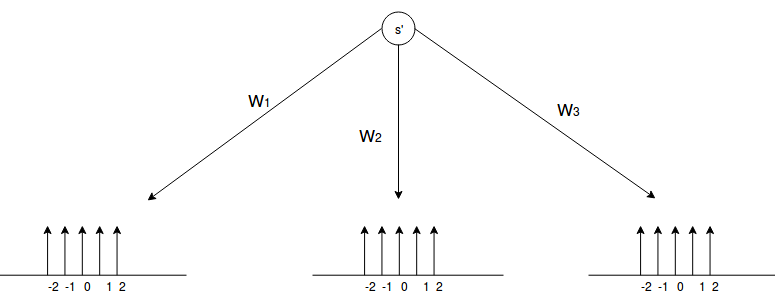
\includegraphics[width=\linewidth]{particles.png}
 \caption{Target Q-distributions of state $s'$.}
 \label{fig:target_distributions}
\end{figure}
Pseudocode of the algorithm is shown in Alg. ~\ref{alg:weighted_updating}. 
\begin{algorithm}[H]
\begin{flushleft}
 \textbf{Input:} A transition $s,a,r,s'$, $\gamma \in [0,1]$, $\alpha \in [0,1]$\\
\end{flushleft}
 \begin{algorithmic}
 
 \For{$j \in 1, \cdots, m$}
 		\State $w_j =\sum_{i=1}^{N} \frac{1}{N} \prod_{a' \neq a} \sum_{x_{a'}^j < x_a^i} \frac{1}{N}$
 \EndFor
 \For{$i \in 1, \cdots, N$}
 		\State $x'^{t}_i(s')= \sum_{j=1}^{m} w_j x'^{t}_i(s',a_j)$ 
 		\State $x^{t+1}_i(s,a) \leftarrow x^{t}_i(s,a) + \alpha (r+\gamma x'^{t}_i(s') - x^{t}_i(s,a))$
 \EndFor
 \end{algorithmic}
 \caption{Weighted Updating}
 \label{alg:weighted_updating}
\end{algorithm}  